\documentclass[11pt,a4paper]{article}

\usepackage[a4paper,margin=1in]{geometry}
\usepackage{graphicx}
\usepackage{booktabs}
\usepackage{float}
\usepackage{hyperref}
\usepackage{xcolor}
\usepackage{listings}
\usepackage{enumitem}
\usepackage{fancyhdr}

\hypersetup{colorlinks=true,linkcolor=blue,urlcolor=blue}

\pagestyle{fancy}
\setlength{\headheight}{14pt}
\fancyhf{}
\lhead{Computer Networks Laboratory}
\rhead{Assignment 3}
\cfoot{\thepage}

\lstdefinestyle{cstyle}{
  language=C,
  basicstyle=\ttfamily\small,
  numbers=left,
  numberstyle=\tiny,
  frame=single,
  breaklines=true,
  showstringspaces=false,
  keywordstyle=\color{blue},
  commentstyle=\color{gray},
  stringstyle=\color{purple}
}
\lstset{style=cstyle}

\setlength{\parskip}{0.5em}
\setlength{\parindent}{0pt}

\begin{document}

\begin{center}
{\LARGE \textbf{Assignment 3: Implementation of HTTP Client using TCP Sockets}}\\[4mm]
Simiyon Vinscent Samuel L\\
Register Number: 3122247001062\\
Submission Date: August 17, 2026\\
GitHub Repository: \url{https://github.com/blackscythe123/PCN-assign}
\end{center}

\vspace{2mm}
\hrule
\vspace{4mm}

\section*{Aim}
To write a plain TCP-socket HTTP client in C that can fetch a page or file from any
web server given its URL, and to check it against a Python \texttt{http.server}
hosting a small set of resources (an HTML page, a text file, a PDF and a JPEG). Along
the way the client also has to measure connection time, download time and throughput
for each request, so the point is as much about instrumenting the socket calls as it
is about getting the GET request right.

\section*{Setting Up the Web Server Files}
\texttt{CN\_Web\_Server/} holds the four files the brief asks for --
\texttt{index.html}, \texttt{notes.txt}, \texttt{sample.pdf} and \texttt{image.jpg} --
served with a plain \texttt{python3 -m http.server 8000}. \texttt{index.html} and
\texttt{notes.txt} are just written by hand. \texttt{sample.pdf} and \texttt{image.jpg}
had no ready-made tool available to generate them (no ImageMagick, no PDF exporter), so
both were built directly: the PDF from its raw object/xref syntax, and the JPEG with a
small from-scratch encoder (real DCT, standard quantisation and Huffman tables) that
produces a genuine 64x64 colour-bar test image. Both were checked with \texttt{file}
and, for the JPEG, with an independent decode script, so they are real, valid files and
not just placeholder bytes with the right extension.

\section*{Part (a): A Generic HTTP Client}
\texttt{http\_client.c} asks the user for a full URL, splits it into host, port and
path, opens a TCP connection, and sends a plain HTTP/1.1 GET with \texttt{Host} and
\texttt{Connection: close}. Because it does not hardcode the host, the exact same
binary works against the local Python server in Part (b) and against a real server on
the internet -- Figure~1 shows it run against \url{http://info.cern.ch/}, whose
646-byte body it downloads and saves byte-for-byte intact.

\begin{lstlisting}[caption={Excerpt of http\_client.c -- parse\_url(): splitting an http:// URL into host, port and path}]
if (strncmp(p, "http://", 7) == 0) {
    p += 7;
} else if (strncmp(p, "https://", 8) == 0) {
    fprintf(stderr, "This client only supports plain http:// URLs.\n");
    return -1;
} else {
    fprintf(stderr, "URL must start with http://\n");
    return -1;
}

/* Everything up to the next '/' is host[:port] */
const char *slash = strchr(p, '/');
const char *hostport_end = slash ? slash : p + strlen(p);

char hostport[MAX_HOST_LEN + 16];
size_t hp_len = (size_t)(hostport_end - p);
memcpy(hostport, p, hp_len);
hostport[hp_len] = '\0';

char *colon = strchr(hostport, ':');
if (colon) {
    *colon = '\0';
    *port = atoi(colon + 1);
    if (*port <= 0) *port = 80;
} else {
    *port = 80;
}
strncpy(host, hostport, host_len - 1);

/* Path is whatever follows the host[:port], default to "/" */
strncpy(path, slash ? slash : "/", path_len - 1);
\end{lstlisting}

\begin{figure}[H]
\centering
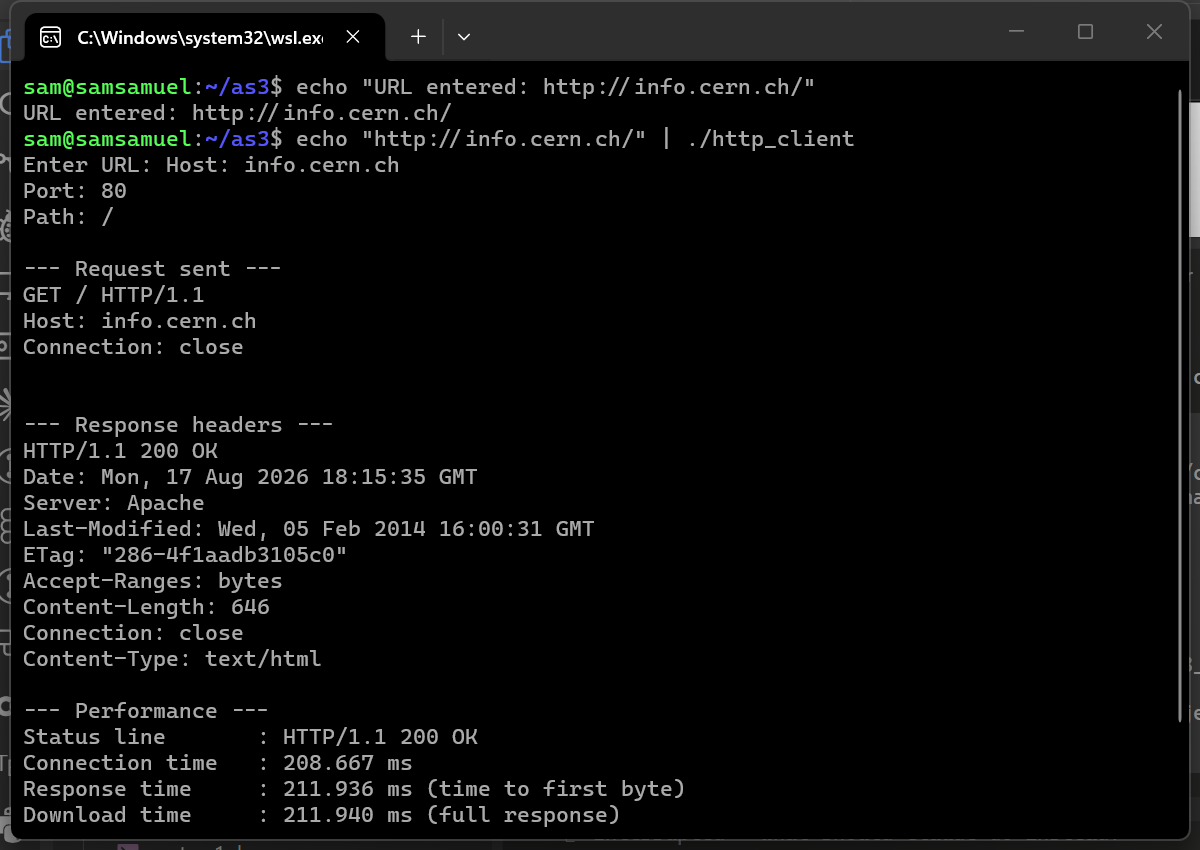
\includegraphics[width=0.85\linewidth]{ss/01_external_http.png}
\caption{http\_client run against a real external URL, http://info.cern.ch/, showing
the parsed host/port/path and the full performance readout.}
\end{figure}

External HTTP tests (mostly for a sanity check that the client is not hardwired to
localhost):

\begin{table}[H]
\centering
\footnotesize
\begin{tabular}{@{}lcrrrrr@{}}
\toprule
URL & Status & Size (B) & Conn. (ms) & TTFB (ms) & Download (ms) & Rate (KB/s) \\
\midrule
info.cern.ch/ & 200 OK & 646 & 184.566 & 186.698 & 186.714 & 3.38 \\
example.com/ & 200 OK & 571 & 5.434 & 10.748 & 11.689 & 47.70 \\
\bottomrule
\end{tabular}
\caption{Part (a) results against real external servers. example.com's body came back
chunked (via Cloudflare); this client does not dechunk, so info.cern.ch -- a plain
Content-Length response -- was used for the clean byte-for-byte check.}
\end{table}

\section*{Part (b): Talking to the Python Web Server}
With \texttt{python3 -m http.server 8000} running inside \texttt{CN\_Web\_Server/}
(Figure~2), the same client was pointed at each of the four hosted files in turn.
Every download came back byte-for-byte identical to the original file (checked with
\texttt{cmp}/\texttt{diff}), and the \texttt{Content-Type} the server reports matches
the file each time (\texttt{text/html}, \texttt{text/plain}, \texttt{application/pdf},
\texttt{image/jpeg}).

\begin{lstlisting}[caption={Excerpt of http\_client.c -- sending the request and timing the response}]
clock_gettime(CLOCK_MONOTONIC, &t_req_sent);
send(sockfd, request, strlen(request), 0);

int got_first_byte = 0;
while ((n = recv(sockfd, buf + total, capacity - total, 0)) > 0) {
    if (!got_first_byte) {
        clock_gettime(CLOCK_MONOTONIC, &t_first_byte);
        got_first_byte = 1;
    }
    total += (size_t)n;
    if (total == capacity) {
        capacity *= 2;
        buf = realloc(buf, capacity);
    }
}
clock_gettime(CLOCK_MONOTONIC, &t_done);

double connect_ms  = elapsed_ms(t_conn_start, t_conn_end);
double response_ms = elapsed_ms(t_req_sent, t_first_byte);   /* time to first byte */
double download_ms = elapsed_ms(t_req_sent, t_done);         /* full transfer */
double throughput_Bps = (double)body_len / (download_ms / 1000.0);
\end{lstlisting}

\begin{figure}[H]
\centering
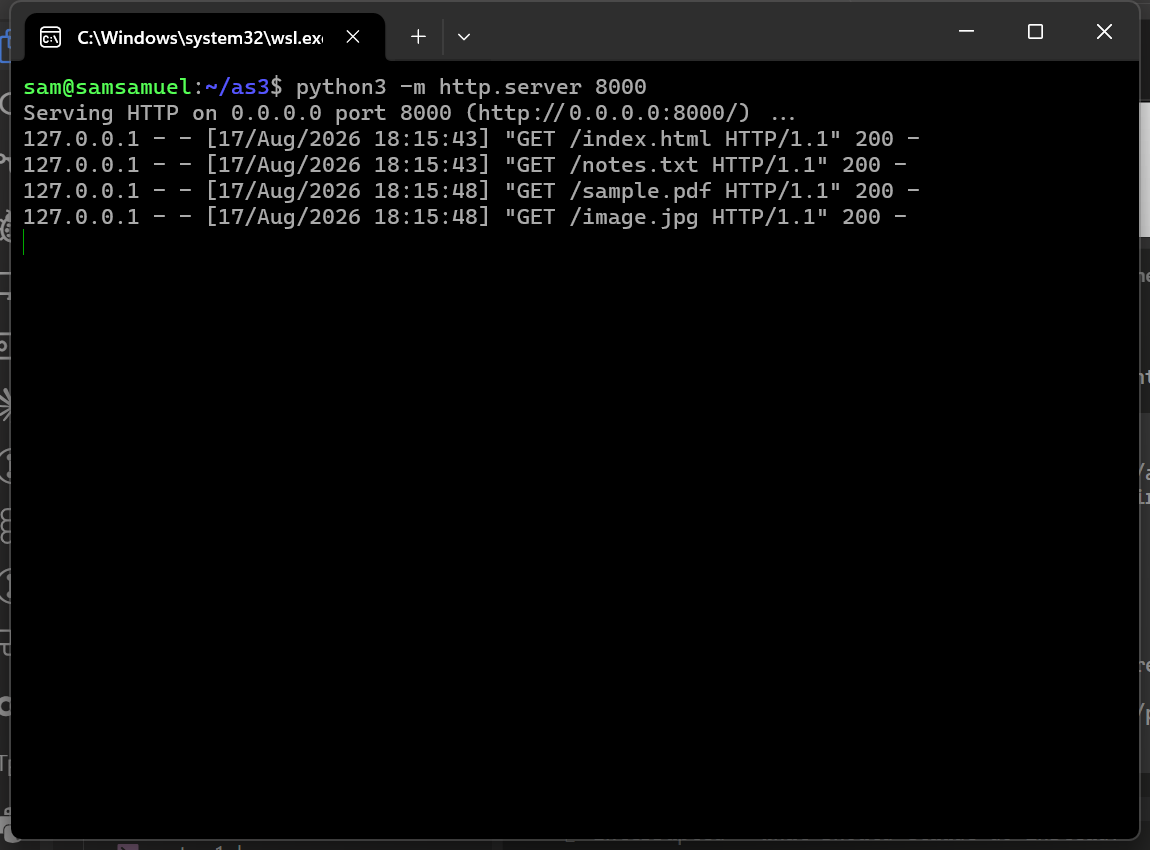
\includegraphics[width=0.85\linewidth]{ss/02_python_server.png}
\caption{The Python http.server terminal, logging each incoming GET as the client
requests it.}
\end{figure}

\begin{figure}[H]
\centering
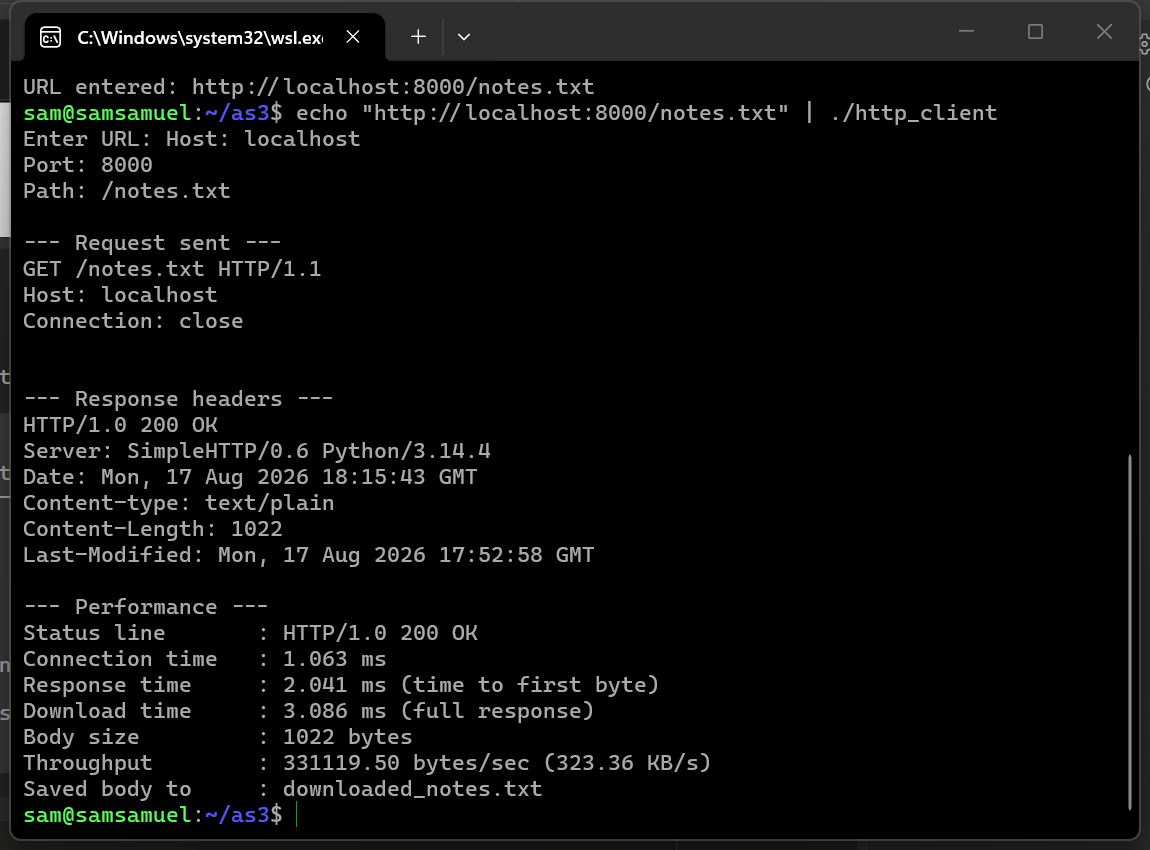
\includegraphics[width=0.85\linewidth]{ss/03_client_html_txt.png}
\caption{http\_client run twice against the local server -- index.html, then
notes.txt.}
\end{figure}

\begin{figure}[H]
\centering
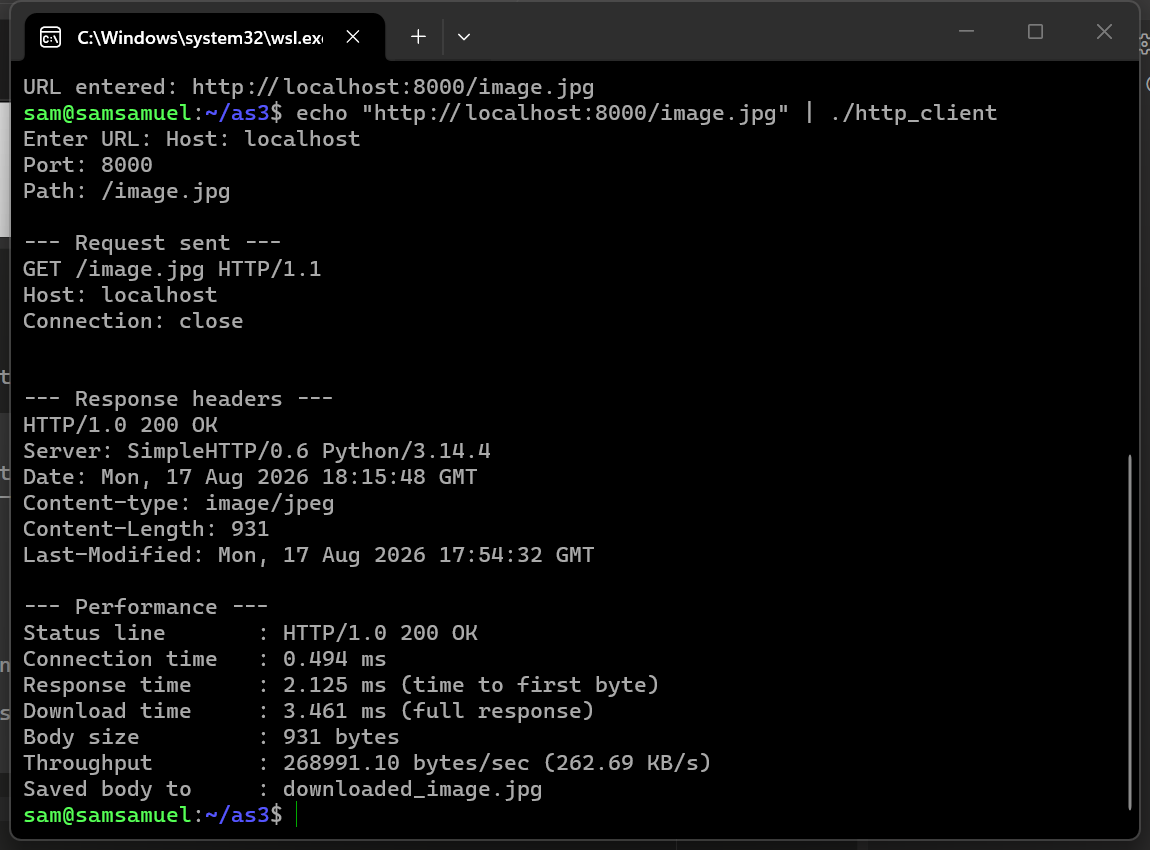
\includegraphics[width=0.85\linewidth]{ss/04_client_pdf_img.png}
\caption{http\_client run twice more -- sample.pdf, then image.jpg -- both saved and
confirmed byte-identical to the originals.}
\end{figure}

\begin{table}[H]
\centering
\footnotesize
\begin{tabular}{@{}lcrrrrr@{}}
\toprule
File & Status & Size (B) & Conn. (ms) & TTFB (ms) & Download (ms) & Rate (KB/s) \\
\midrule
index.html & 200 OK & 168 & 0.137 & 4.317 & 6.220 & 26.38 \\
notes.txt & 200 OK & 1022 & 0.255 & 2.442 & 3.559 & 280.41 \\
sample.pdf & 200 OK & 642 & 0.276 & 2.177 & 3.169 & 197.86 \\
image.jpg & 200 OK & 931 & 0.509 & 1.930 & 3.066 & 296.50 \\
missing file & 404 & 460 & 0.126 & 1.512 & 1.614 & 278.31 \\
\bottomrule
\end{tabular}
\caption{Part (b) results, Python http.server on localhost:8000. All four real files
matched their originals byte-for-byte.}
\end{table}

The numbers are small because everything is on loopback -- they mostly show syscall
overhead rather than anything about real network bandwidth, but the instrumentation
itself (connect time, time-to-first-byte, full download time, throughput) is doing
exactly what it should.

The last row is a request for a file that does not exist on the server. The brief
does not require handling this case specially, and the client does not try to -- it
gets back \texttt{HTTP/1.0 404 File not found} with Python's usual small HTML error
page and just saves that body like it would any other response.

\section*{Bonus: Secure HTTPS Client (Optional Advanced Program)}
The optional part was attempted and works: \texttt{https\_client.c} does the same job
as \texttt{http\_client.c} but over TCP + OpenSSL on port 443 -- TLS handshake,
certificate verification (chain and hostname), an encrypted GET, and timing for the
TCP connect, the SSL handshake, and the round trip to the first response byte.

\begin{lstlisting}[caption={Excerpt of https\_client.c -- TLS handshake and certificate verification}]
SSL_CTX_set_verify(ctx, SSL_VERIFY_PEER, NULL);
SSL_CTX_set_default_verify_paths(ctx);

SSL *ssl = SSL_new(ctx);
SSL_set_fd(ssl, sockfd);
SSL_set_tlsext_host_name(ssl, host);  /* SNI */
SSL_set1_host(ssl, host);             /* also check the cert name matches host */

clock_gettime(CLOCK_MONOTONIC, &t_ssl_start);
SSL_connect(ssl);
clock_gettime(CLOCK_MONOTONIC, &t_ssl_end);

long verify_result = SSL_get_verify_result(ssl);
printf("Certificate verification: %s\n",
       (verify_result == X509_V_OK) ? "OK (trusted chain + hostname match)"
                                     : X509_verify_cert_error_string(verify_result));
\end{lstlisting}

\begin{figure}[H]
\centering
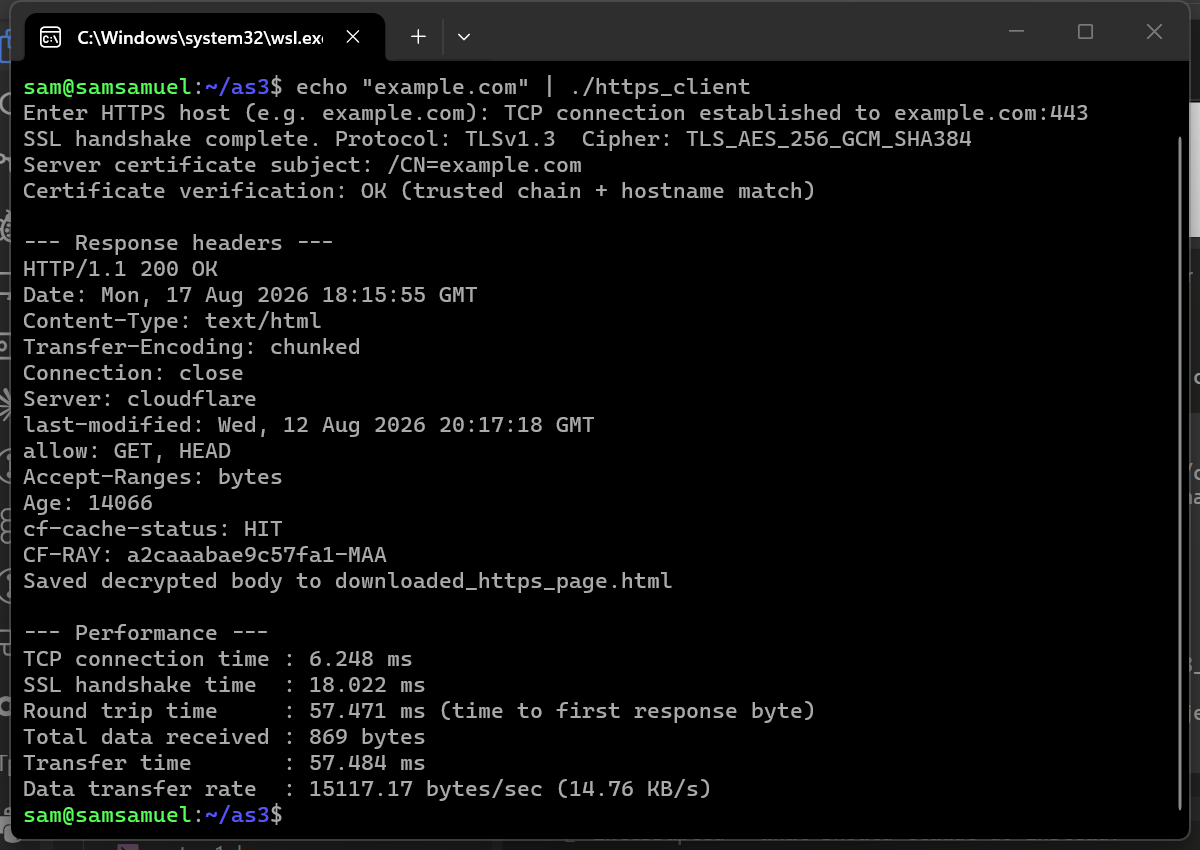
\includegraphics[width=0.85\linewidth]{ss/05_https_advanced.png}
\caption{https\_client run against a real HTTPS site -- TLS handshake, certificate
verification and the encrypted GET all succeeding.}
\end{figure}

\begin{table}[H]
\centering
\footnotesize
\begin{tabular}{@{}lccrrr@{}}
\toprule
Host & TLS / Cipher & Cert & Handshake (ms) & TTFB (ms) & Rate (KB/s) \\
\midrule
example.com & TLSv1.3 / AES-256-GCM & OK & 22.872 & 84.610 & 10.02 \\
www.google.com & TLSv1.3 / AES-256-GCM & OK & 35.935 & 84.841 & 926.64 \\
\bottomrule
\end{tabular}
\caption{Optional HTTPS client results against two real servers.}
\end{table}

\section*{Learning Outcome}
\begin{itemize}
\item Writing a URL parser by hand made it obvious how much a browser normally hides --
default ports, missing paths, and the scheme check all need explicit code, not just a
happy-path GET.
\item Timing connection time separately from time-to-first-byte and full download time
made it clear these are genuinely different numbers even on loopback -- the connect
was consistently the cheapest part, first-byte latency the biggest chunk.
\item Building sample.pdf and image.jpg from scratch, without any image or PDF tool
available, was a good forced lesson in file formats: a PDF is just a text-ish object
graph with an offset table, and a JPEG's structure is far more approachable once you
strip it down to a flat-colour block with no interesting AC coefficients.
\end{itemize}

\end{document}
